\chapter{Face and Body Pose Tracking} \label{applications}

Chapter \ref{system} presented an integrated vision system for \RD{}, and Chapter \ref{depthcolor} showed 
that it is possible to build new camera representations on top of it. Along with capturing and handling images, 
a vision system should be able to retrieve information from them. This chapter integrates two algorithms in the 
field of object detection and tracking that let the system gather information about humans in the 
camera's surroundings. 

Section \ref{facetracker} presents a face tracking algorithm that operates on the depth-color images introduced 
in Chapter \ref{depthcolor}. This algorithm uses the depth information to segment the person of interest from 
the background and consequently reduce the number of false positives detected by a traditional face detector.
The algorithm is shown to be robust to different face positions and orientations. 

Section \ref{bodyposetracker} introduces a representation for the Microsoft's Kinect camera and integrates an
open source framework that uses the Kinect's images to detect and track a person's body pose. The algorithm 
implemented in this framework operates on the depth images captured by the Kinect and outputs a body 
skeleton indicating the position and orientation of various joints in the human body. 

In this chapter, the Kinect becomes the second depth-color camera that forms part of the integrated vision 
system. In conjunction with the two tracking algorithms, this serves to point out the new importance of these 
sensors in the field of computer vision. 


\section{Face Tracker} \label{facetracker}
The images from a depth-color camera can be used to get better results from traditional face detection 
algorithms. The false positives from such algorithms come in part from pixels in the background that are 
thought to be faces. With the depth-color images, the depth information can be used to remove pixels from the 
background based on distance thresholds.

The \FaceTracker{} class implements an algorithm that uses the Viola-Jones object detection framework 
\cite{Viola} to find faces in depth-color images. Furthermore, after detecting the faces it uses the Camshift
(Continuously Adaptive Mean Shift) algorithm \cite{BradskiCamshift} to track them based on color information. 
The \FaceTracker{} uses the OpenCV library's implementations of the Viola-Jones and Camshift algorithms. 
\footnote{OpenCV implements the extended version of the Viola-Jones detector described by Lienhart and 
Maydt \cite{Lienhart}.}

The idea of the \FaceTracker{} algorithm consists of discarding the pixels in the fused color image that are
below or above certain depth thresholds. The value for these pixels are replaced with a zero value (a black 
pixel) creating uniform areas in the image that do not contain color information. Figure \ref{fusion} already
showed an example of a fused color image after thresholding based on depth. It revealed that this technique
can successfully segment the object of interest from the background, given that there is a significant distance
between the two.

Table \ref{facetrackeralgorithm} describes the algorithm of the \texttt{find\-Fac\-es} method, the main method 
of the face tracker class. This method performs the task of running the Viola-Jones detector and the Camshift 
tracker, and integrating the results from both algorithms.

\begin{table}[ht]
\caption{Algorithm for the \texttt{findFaces} method in \FaceTracker{}}
\begin{center}
\begin{tabular}{ l l }
\hline
\multicolumn{2}{l}{\texttt{FIND\_FACES (faceStream, successThreshold):}} \\
1 & \texttt{Run Viola-Jones face detector;} \\
2 & \texttt{{\bf If} face is detected} \\
3 & \hspace{0.6cm} \texttt{\bf Then:} \\
4 & \hspace{1.2cm} \texttt{Add face to faceStream;} \\
5 & \hspace{1.2cm} \texttt{{\bf If} the number of consecutive found faces} \\
- & \hspace{1.2cm} \texttt{is larger than successThreshold} \\
6 & \hspace{1.8cm} \texttt{\bf Then:} \\
7 & \hspace{2.4cm} \texttt{Initialize Camshift with the detection} \\
- & \hspace{2.4cm} \texttt{window of the found face} \\
8 & \hspace{0.6cm} \texttt{\bf Else:} \\
9 & \hspace{1.2cm} \texttt{{\bf If} faceStream contains a face for the last image} \\
- & \hspace{1.2cm} \texttt{and Camshift has been initialized} \\
10 & \hspace{1.8cm} \texttt{\bf Then:} \\
11 & \hspace{2.4cm} \texttt{Run the Camshift tracker;} \\
12 & \hspace{2.4cm} \texttt{{\bf If} face is successfully tracked} \\
13 & \hspace{3.0cm} \texttt{\bf Then:} \\
14 & \hspace{3.6cm} \texttt{Add face to faceStream;} \\
\hline
\end{tabular}
\end{center}
\label{facetrackeralgorithm}
\end{table}

The algorithm gives priority to the Viola-Jones detector over the Camshift tracker, mainly because Camshift 
only relies on tracking a patch of pixels with color distribution similar to that of a reference patch. Furthermore, 
this design follows the assumption that a person, the object of interest for the \FaceTracker{}, will be facing the 
camera most of the time, prompting in that way a high rate of successful face detections. Therefore, the 
detector is ran on every call to \texttt{find\-Fac\-es} (line 1), while the tracker is used as a backup for when the 
detector fails to find a face (line 11). 

The Camshift tracker needs to ``initialized'' before it can track a face (line 7). This initialization consists of 
building a histogram of the color information in a given reference window. The color information is the hue 
channel of the image and the reference window is the face detection window outputted by the Viola-Jones 
detector. Afterwards, every run of the tracker (line 11) calculates the back projection of the input image's hue 
channel using the reference histogram, and uses that to find the new location of the reference face. It is not
necessary to reinitialize the tracker on every successful detection because on consecutive image frames 
the position of the face does not change drastically. However, after some time the information in the reference
histogram might need to be refreshed, making necessary to reinitialize the tracker with a new face detection
window (lines 5 to 7).

The faces found by the \FaceTracker{} algorithm are added to a \FaceStream{} object (lines 4 and 14). The 
\FaceStream{} class extends \Stream{} and is similar in concept to the image stream representation discussed
in Section \ref{imagestream}. In this case, the stream uses objects of the type \List{} as buffer objects. In these 
lists the stream can store multiple instances of the \Face{} class, a simple data structure that holds the face's 
position and dimension. The advantage of storing the found faces in a face stream is that the user can 
define other algorithms based on the stored result of consecutive calls to \texttt{find\-Fac\-es}.

Table \ref{facetrackermethods} lists the methods of this class. The \texttt{de\-tect\-Fac\-es}, 
\texttt{in\-i\-tial\-ize\-Track\-ers}, and \texttt{track\-Fac\-es} methods are called by \texttt{find\-Fac\-es} to 
run the Viola-Jones detector, initialize Camshift, and run the Camshift tracker, respectively. The 
\texttt{get\-Fac\-es\-In\-Fused} method can be used to access the faces found on the last call to 
\texttt{find\-Fac\-es}. The actual face stream is accessed through the \texttt{get\-Fac\-es\-In\-Fused\-Stream} 
method.

\begin{table}[ht]
\caption{Public methods in the \FaceTracker{} class}
\begin{center}
\begin{tabular}{| l |}
	\hline 
	\multicolumn{1}{| c |}{\FaceTracker{}} \\
	\hline \hline
	\texttt{findFaces} \\
	\texttt{detectFaces} \\
	\texttt{initializeTrackers} \\
	\texttt{trackFaces} \\
	\texttt{mapFace} \\
	\texttt{getFacesInFused} \\
	\texttt{getFacesInColor} \\
	\texttt{getFacesInFusedStream} \\
	\texttt{getFacesInColorStream} \\
	\texttt{drawFaceInColor} \\
	\texttt{drawFaceInFused} \\
	\texttt{findFaceInterior} \\
	\texttt{mapFaceInterior} \\
	\hline
\end{tabular}
\end{center}
\label{facetrackermethods}
\end{table}

Furthermore, since the \DepthColorFusion{} object contains the mapping from pixels in the depth image to 
pixels in the color image (see Section \ref{depthcolorfusion}), it is possible to know the position of the face in 
the original color image. The \texttt{map\-Face} method is used to map faces from the fused color image to the 
original color image. This method is called automatically by the face tracker in order to provide an additional 
stream of faces. The \texttt{get\-Fac\-es\-In\-Col\-or} and \texttt{get\-Fac\-es\-In\-Col\-or\-Stream} methods
are used to access the faces in the original color image. 

The face tracker takes advantage of this mapping by providing the capability of detecting the 
eyes, nose, and mouth of a face using the Viola-Jones detector. Since the fused color image does not provide 
the necessary resolution to detect face parts, the face tracker uses the mapped face to run the detector 
on the region of interest of the original color image. The \texttt{find\-Face\-In\-te\-ri\-or} method performs this 
operation, and the \texttt{map\-Face\-In\-te\-ri\-or} method can be used to map the positions of the eyes, nose, 
and mouth back to the depth-color image.

Figure \ref{facetrackersequence} shows a sequence of fused color images that have passed through the
\FaceTracker{}'s algorithm. The red squares indicate the position and dimension of the face that was found 
on each of the images. Once the face tracker detects a person facing the camera, it can start tracking the face
through different head movements. The sequence of images shows that the algorithm is robust to change in 
face position (including distance from the camera) and orientation.

\begin{figure}[t]
\center
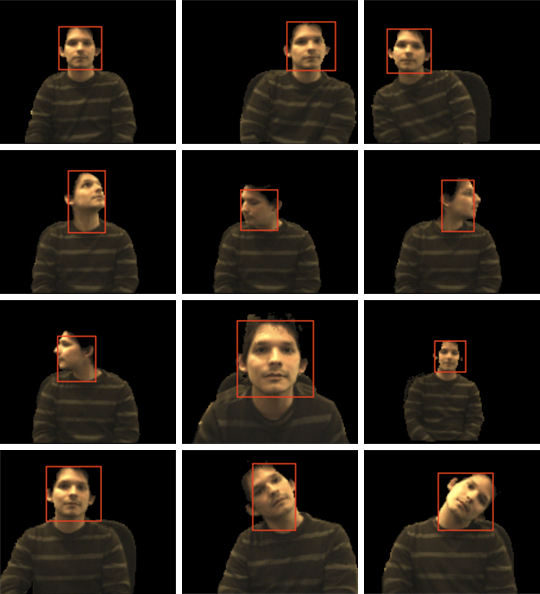
\includegraphics[width = 10cm]{facetracker.png}
\caption[Output of the \FaceTracker{}'s algorithm]{Output of the \FaceTracker{}'s algorithm on a sequence 
of depth-color images. The red squares indicate the position and dimension of the faces.}
\label{facetrackersequence}
\end{figure}


\section{Body Pose Tracker} \label{bodyposetracker}
The vision system also provides a way of tracking the body pose of a person. This is achieved through the
OpenNI open source framework, which provides support for detecting and tracking the body of a human 
in depth images \cite{OpenNI}. OpenNI achieves this by attempting to fit a skeleton on a potential human body. 
The information about the skeleton's joints is used to extract the position and orientation of the body.

The OpenNI module that contains the skeleton fitting capabilities is designed to work exclusively with 
PrimeSense derived sensors \cite{PrimeSensor, NITE}. An example of such sensor is the Microsoft's Kinect 
camera. Similar to the depth-color camera setup described in Chapter \ref{depthcolor}, the Kinect is designed
to capture depth and color images, everything on a single piece of hardware. The Kinect's images can be 
retrieved using the PrimeSense interface provided by OpenNI.

In order to take advantage of OpenNI's body tracking support, the vision system introduces the \KinectCam{} 
class. This class serves both as a representation of the Kinect camera and an interface to the OpenNI 
framework. The \KinectCam{} class is implemented following the same structure as the \ColorCam{} and 
\SwissRangerCam{} classes (see Sections \ref{colorcam} and \ref{swissrangercam}). The \KinectJavaAcquire{}
class establishes the Java interface to OpenNI and as such is used to retrieve the images and body 
skeleton information. The \KinectPacketHandler{} class receives image and skeleton data that is transferred 
over the network. The \KinectReceiver{} uses instances of the two previous classes to handle the data streams 
from the Kinect. A Kinect receiver is used by the \KinectCam{} class to gain access to the image and 
skeleton data. 

This design reveals that, in the \RD{} environment, the Kinect camera is seen not only as a sensor that 
provides depth and color images, but also as a sensor that provides body skeleton data for every image 
frame. The skeleton data is represented with an object of type \KinectSkeleton{}. This object contains the 
position and orientation of every joint in the body skeleton generated by OpenNI. The Kinect receiver handles
the skeleton objects using an instance of the \KinectSkeletonStream{} class, a subtype of \Stream{}. The 
\KinectSkeletonStream{} class represents a sequence of detected body poses, and its design is similar to the 
design of the \FaceStream{} class discussed in Section \ref{facetracker}.

Table \ref{kinectcammethods} lists the methods that the \KinectCam{} class adds to the base camera
representation. The \texttt{get\-Skel\-e\-tons} method further exemplifies the idea that in this system the Kinect
captures image and body skeleton data. The \texttt{cre\-ate\-Dis\-play} method is used to create a color 
visualization of the raw depth data, and the \texttt{thresh\-old} method serves to threshold the values of the
depth image.

\begin{table}[ht]
\caption{Public methods in the \KinectCam{} class}
\begin{center}
\begin{tabular}{| l |}
	\hline 
	\multicolumn{1}{| c |}{\KinectCam{}} \\
	\multicolumn{1}{| c |}{{\small \texttt{extends} \Camera{}}} \\
	\hline \hline
	\texttt{getColor} \\
	\texttt{getDepth} \\
	\texttt{getSkeletons} \\
	\texttt{getDepthDisplay} \\
	\texttt{getColorView} \\
	\texttt{getDepthView} \\
	\texttt{createDisplay} \\
	\texttt{threshold} \\
	\hline
\end{tabular}
\end{center}
\label{kinectcammethods}
\end{table}

Figure \ref{bodyposetrackersequence} shows a sequence of depth images captured with the Kinect camera
along with superimposed red skeletons that illustrate the output of OpenNI's body tracking algorithm. As it has 
been seen before, thresholding the image based on the depth values can segment the body of a person from 
the background assuming there is a significant distance between the two. The top left image shows the position
of the body that is required to calibrate and start the tracking algorithm. The other images show that the 
algorithm is robust to different body positions and orientations. 

One of the principal advantages of the body skeleton data is that it can be used as input to gesture recognition
algorithms. For example, the skeleton can provide information about the position of a person's arms with 
respect to the rest of the body. This information can be used to train algorithms that classify certain arm 
movements into gestures, making possible to recognize, for example, an arm waving, pointing, or reaching out. 

\begin{figure}[t]
\center
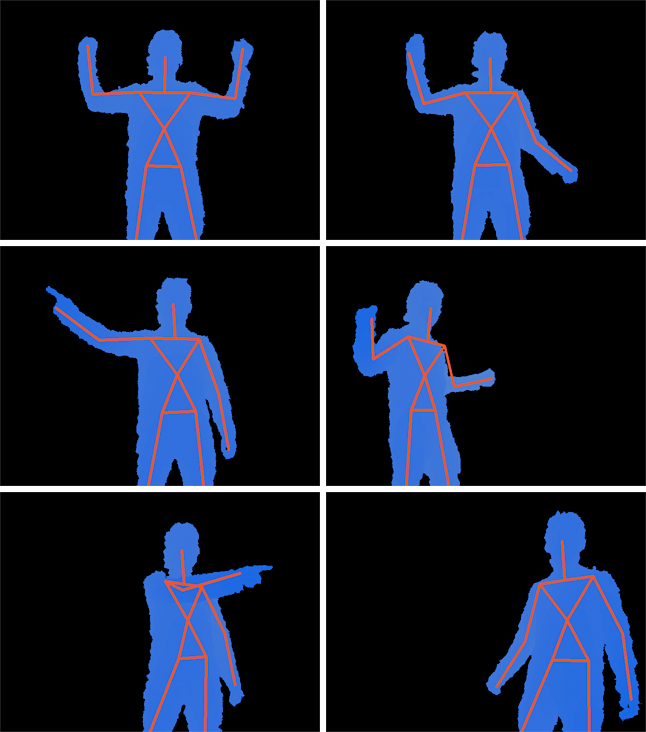
\includegraphics[width = 10cm]{bodyposetracker.png}
\caption[Output of OpenNI's body pose tracking algorithm]{Output of OpenNI's body pose tracking 
algorithm on a sequence of depth images. The red lines indicate the position of the skeleton's joints.}
\label{bodyposetrackersequence}
\end{figure}